\documentclass[11pt]{article}
\usepackage[review]{acl}
\usepackage{times}
\usepackage{latexsym}
\usepackage[T1]{fontenc}
\usepackage{microtype}
\usepackage{booktabs}
\usepackage{xcolor}
\usepackage{tikz}

\newcommand{\lead}[1]{\textcolor{red}{\textbf{[LEAD: #1]}}}
\newcommand{\lbl}[1]{\textsc{#1}}
\newcommand{\gl}[1]{`#1'}

\title{What Form Cannot Tell: Resemblance, the Intermediate Stage,\\and Wiktionary's Inherited and Learned Labels in 17 Languages}

\author{Anonymous submission}

\begin{document}
\maketitle

\begin{abstract}
Many languages have two layers of words from one ancestor: words inherited over centuries, and words borrowed back later from its books (Hindi \textit{tadbhava} and \textit{tatsama}; Spanish inherited and learned Latin words). Wiktionary labels tens of thousands of words this way, and such labels have been used to train classifiers. We ask what a model learns from them, in 17 language pairs and 13,128 sampled pages. \textbf{Form is a shortcut to the label}: minimal models reach macro-F1 of 0.86 to 0.96 for seven languages descended from Sanskrit and 0.75 to 0.91 for seven Romance languages, but are right on only 10\% and 19\% of the items where label and resemblance disagree. \textbf{Those labels are not noise}: specialists side with Wiktionary on 45 of 48 such items, the model on 22. \textbf{The intermediate stage explains the failure and does not repair it}: for 84\% of the hard inherited words the Middle Indo-Aryan form is itself almost the Sanskrit form, and neither a linear model nor two character Transformers gain from seeing it. Reweighting, word meaning and a dictionary record lift accuracy on the hard items from 10\% to 53\%, and no further. For such words the route is a matter of record, not of form. A lookup of 48 Hindi and Bengali lemmas in four dictionaries, automated under rules frozen in advance and partly checked by hand, assigned a route to 26 of 58 senses. Learned labels remain unvalidated: a score on them measures agreement with Wiktionary, not historical accuracy.
\end{abstract}

\begin{figure*}[t]
\centering
\begin{tikzpicture}[x=1cm,y=1cm]
\draw[rounded corners=3pt,fill=black!6] (0.00,0) rectangle (3.05,2.35);
\node[font=\footnotesize\bfseries,align=center,text width=3.0cm] at (1.525,1.98) {Form predicts\\the label};
\node[font=\Large\bfseries] at (1.525,1.3) {0.86--0.96};
\node[font=\scriptsize,align=center,text width=3.0cm] at (1.525,0.5) {macro-F1, Sanskrit family;\\Romance 0.75--0.91 (\S\ref{sec:baseline})};
\draw[rounded corners=3pt,fill=black!6] (3.20,0) rectangle (6.25,2.35);
\node[font=\footnotesize\bfseries,align=center,text width=3.0cm] at (4.725,1.98) {\ldots but not\\the hard items};
\node[font=\Large\bfseries] at (4.725,1.3) {10\% \textperiodcentered{} 19\%};
\node[font=\scriptsize,align=center,text width=3.0cm] at (4.725,0.5) {right where label and\\resemblance disagree (\S\ref{sec:baseline})};
\draw[rounded corners=3pt,fill=black!6] (6.40,0) rectangle (9.45,2.35);
\node[font=\footnotesize\bfseries,align=center,text width=3.0cm] at (7.925,1.98) {The labels follow\\a dictionary};
\node[font=\Large\bfseries] at (7.925,1.3) {46\% vs 10\%};
\node[font=\scriptsize,align=center,text width=3.0cm] at (7.925,0.5) {matching form listed: called\\inherited vs learned (\S\ref{sec:link})};
\draw[rounded corners=3pt,fill=black!6] (9.60,0) rectangle (12.65,2.35);
\node[font=\footnotesize\bfseries,align=center,text width=3.0cm] at (11.125,1.98) {The missing link\\is no cure};
\node[font=\Large\bfseries] at (11.125,1.3) {84\%};
\node[font=\scriptsize,align=center,text width=3.0cm] at (11.125,0.5) {intermediate form unchanged\\in hard inherited words (\S\ref{sec:link})};
\draw[rounded corners=3pt,fill=black!6] (12.80,0) rectangle (15.85,2.35);
\node[font=\footnotesize\bfseries,align=center,text width=3.0cm] at (14.325,1.98) {Specialists back\\Wiktionary};
\node[font=\Large\bfseries] at (14.325,1.3) {45 of 48};
\node[font=\scriptsize,align=center,text width=3.0cm] at (14.325,0.5) {hard items; the model agrees\\with them on 22 (\S\ref{sec:link})};
\end{tikzpicture}
\caption{The findings at a glance.}
\label{fig:cards}
\end{figure*}

\section{Introduction}

A modern Indo-Aryan word with a Sanskrit etymon can have one of several histories. It may have been \textbf{inherited} through the Middle Indo-Aryan stages, with the sound changes of those stages (\textit{tadbhava}). It may be a \textbf{learned} borrowing taken later from Sanskrit as a prestige language (\textit{tatsama}), or a \textbf{semi-learned} borrowing whose form was partly adapted (\textit{ardhatatsama}, or semi-tatsama) \citep[\S111]{chatterji1926}. As \citeauthor{chatterji1926} notes, \textit{tatsama} in modern use describes the form of a word and not the way it entered the language, so we state our categories as routes. The distinction matters for historical phonology, because learned words do not show the regular changes, and it is a natural target for computational attribution.

For Romance, \citet{cristea2021inherited} trained classifiers to separate inherited from borrowed Latin words, with labels taken from Wiktionary etymology templates. The same kind of label exists for Indo-Aryan. On 10 October 2026 the English Wiktionary category for Hindi learned borrowings from Sanskrit held 1,337 pages, the semi-learned category 98, and the category of terms inherited from Sanskrit 2,241; the Bengali categories held 1,075, 44 and 1,045 pages. These labels are edited by volunteers, and their accuracy is not known.

Before such labels are used to train or to evaluate a model, it is worth asking what a model can learn from them. The route of a word is a claim about a path. An inherited word passed through an intermediate stage, Middle Indo-Aryan or Old French, and carries the changes of that stage; a learned word did not. The usual input to a classifier is the modern word and the ancestor form, the two ends of the path, and not the stage between them. \textbf{We ask how far resemblance to the ancestor explains Wiktionary's labels, where it fails, and whether the intermediate stage or a dictionary can decide the cases where it fails.} This paper studies the labels; its models are minimal baselines and two neural models, one of them pretrained.

The question is an instance of a familiar one. A model can score well on a test set by a cue that goes with the label and is not the property that the label names. In natural language inference, a classifier that sees only the hypothesis recovers much of the label \citep{gururangan2018annotation}, and models that adopt heuristics which hold for frequent example types fail on a controlled set where the heuristics break down \citep{mccoy2019right}. Here the cue is resemblance to the ancestor form, and the property is the path that a word took. We follow that work in reporting the score separately on the items where cue and label disagree, and we go one step further in asking, with dictionaries, intermediate forms and specialists' judgements, whether the labels on those items are right.

Figure~\ref{fig:cards} gives the findings at a glance, and Figure~\ref{fig:grid} shows the central one. Two further parts show that the labels are thinly sourced and hard to check independently: an audit of how the routes are recorded (\S\ref{sec:audit}), and a study of 48 Hindi and Bengali lemmas in four dictionaries (\S\ref{sec:why}; Appendix~\ref{sec:method}).

The audit covers 13,128 pages and gives sample proportions; their intervals are in Appendix~\ref{app:denominators} and the supplementary tables. The source-grounded study is small and was stratified by hand to over-sample hard cases, so for it \textbf{we report raw counts, and no count estimates a rate for Hindi or Bengali vocabulary.} Two small parts compare labels with specialists' judgements, for basic vocabulary; no part establishes more generally which labels are historically correct.

\begin{figure}[t]
\centering
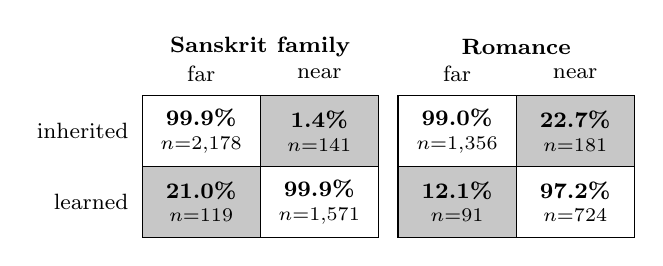
\begin{tikzpicture}[x=1cm,y=1cm,font=\footnotesize]
\node[anchor=east] at (-0.05,1.35) {inherited};
\node[anchor=east] at (-0.05,0.45) {learned};
\node[font=\footnotesize\bfseries] at (1.50,2.42) {Sanskrit family};
\node at (0.75,2.08) {far}; \node at (2.25,2.08) {near};
\draw[fill=white] (0.00,0.90) rectangle (1.50,1.80);
\node[align=center] at (0.75,1.35) {\textbf{99.9\%}\\[-1pt]{\scriptsize $n$=2,178}};
\draw[fill=black!22] (1.50,0.90) rectangle (3.00,1.80);
\node[align=center] at (2.25,1.35) {\textbf{1.4\%}\\[-1pt]{\scriptsize $n$=141}};
\draw[fill=black!22] (0.00,0.00) rectangle (1.50,0.90);
\node[align=center] at (0.75,0.45) {\textbf{21.0\%}\\[-1pt]{\scriptsize $n$=119}};
\draw[fill=white] (1.50,0.00) rectangle (3.00,0.90);
\node[align=center] at (2.25,0.45) {\textbf{99.9\%}\\[-1pt]{\scriptsize $n$=1,571}};
\node[font=\footnotesize\bfseries] at (4.75,2.42) {Romance};
\node at (4.00,2.08) {far}; \node at (5.50,2.08) {near};
\draw[fill=white] (3.25,0.90) rectangle (4.75,1.80);
\node[align=center] at (4.00,1.35) {\textbf{99.0\%}\\[-1pt]{\scriptsize $n$=1,356}};
\draw[fill=black!22] (4.75,0.90) rectangle (6.25,1.80);
\node[align=center] at (5.50,1.35) {\textbf{22.7\%}\\[-1pt]{\scriptsize $n$=181}};
\draw[fill=black!22] (3.25,0.00) rectangle (4.75,0.90);
\node[align=center] at (4.00,0.45) {\textbf{12.1\%}\\[-1pt]{\scriptsize $n$=91}};
\draw[fill=white] (4.75,0.00) rectangle (6.25,0.90);
\node[align=center] at (5.50,0.45) {\textbf{97.2\%}\\[-1pt]{\scriptsize $n$=724}};
\end{tikzpicture}
\caption{Accuracy of the form-based model B3 (\S\ref{sec:baseline}) by Wiktionary's label and by distance of the word from the ancestor form (far: at least 0.5; near: at most 0.15). Shaded: the dissociated items, where label and resemblance disagree.}
\label{fig:grid}
\end{figure}

\section{Related Work}

\citet{cristea2021inherited} is the closest study in design: it discriminates inherited from borrowed Latin words in Romance languages, using Wiktionary templates as labels. For Indo-Aryan, \citet{cathcart2020disentangling} model the sound changes from Old Indo-Aryan etyma to their reflexes, with data taken from \citeauthor{turner1966cdial}'s comparative dictionary, and they state that they do not model contact. \citet{arora2023jambu} compile a database for South Asian historical linguistics that includes the same dictionary, and \citet{arora2022computational} survey the field and identify scattered data as its main obstacle. \citet{list2024openproblems} lists the detection of contact layers among the hard open problems of computational historical linguistics. \citet[\S4.1]{kanojia2021thesis} discusses the tatsama and tadbhava distinction in the context of cognate detection for Indian languages. \citet{wu2020computational} parse Wiktionary's etymologies at scale and predict etymological relations from them. \citet{miller2020lexical} detect borrowings from the wordlist of a single language and conclude that phonological and phonotactic clues alone are often not sufficient.

In the sources that we searched, we did not find a computational classifier that is evaluated on these historical transmission categories for Indo-Aryan, and we did not find a study that audits Wiktionary's route labels across languages or checks them against dictionaries or against the intermediate stage. This statement is bounded by our search and is not a claim that no such work exists. Where the studies above ask whether such labels can be predicted, we ask what a model that predicts them has learned. In that respect the paper belongs with work on annotation artifacts and fallible heuristics in other tasks \citep{gururangan2018annotation,mccoy2019right}, with one difference: there the diagnostic set is built so that its labels are known, and here the labels on the diagnostic items are themselves in question and have to be checked against outside sources. Table~\ref{tab:prior} compares the tasks (Appendix~\ref{app:prior}).

\begin{table*}[t]
\centering\footnotesize
\begin{tabular}{p{0.14\textwidth}p{0.23\textwidth}p{0.26\textwidth}p{0.25\textwidth}}
\toprule
\textbf{Work} & \textbf{Task} & \textbf{Data and method} & \textbf{Relation to this paper} \\
\midrule
\citet{wu2020computational} & Predict the etymological relation of a word, over the etymology types and languages of Wiktionary; model word emergence & A parser for Wiktionary's etymologies; prediction against a baseline & Uses Wiktionary's relations as the reference. We ask what agreement with two of those relations shows. \\
\addlinespace
\citet{cristea2021inherited} & Separate inherited from borrowed Latin words in six Romance languages & Wiktionary templates, and a Romanian dictionary; character n-grams of the word, the etymon and their alignment; spelling and phonetic versions & The same task and label source. We add eleven further languages, the items where label and resemblance disagree, and checks against outside sources. \\
\addlinespace
\citet{miller2020lexical} & Detect borrowings in the wordlist of one language & Language models over the sounds of words & Loans from any source, without an ancestor form. Its conclusion that such clues are often not sufficient agrees with ours. \\
\addlinespace
\citet{cathcart2020disentangling} & Model sound change from Old Indo-Aryan etyma to modern reflexes; subgrouping & Turner's comparative dictionary; a neural model & Models inherited change and states that contact is not modelled. We study the boundary that it sets aside. \\
\addlinespace
\citet{bouchardcote2013automated} & Reconstruct the word forms of protolanguages & A probabilistic model of sound change over a tree of 637 Austronesian languages, compared with a specialist's reconstructions & Reconstructs forms. We reconstruct neither forms nor routes. \\
\midrule
This paper & Test what a score on inherited and learned labels shows & 17 language pairs; form-based baselines; a dictionary, intermediate forms and two expert sources on the hard items; a blind dictionary study of 48 lemmas & \\
\bottomrule
\end{tabular}
\caption{The closest prior work and this paper. Descriptions follow each work's own abstract or text.}
\label{tab:prior}
\end{table*}

\section{A Cross-Lingual Audit of the Labels}
\label{sec:audit}

\paragraph{Design.} A language pair is a modern language and an ancestor from which it has both inherited words and learned borrowings. For each pair Wiktionary has up to three categories: learned borrowings, semi-learned borrowings, and inherited terms. We fixed 32 candidate pairs and eight measures in a plan that was frozen, with a recorded hash, before any category size or page was retrieved. A pair was included if its learned and inherited categories each held at least 100 pages. Seventeen pairs passed (Table~\ref{tab:audit}); the 15 that failed include Persian, Irish, Russian and Japanese. From each category we took up to 400 pages in the order of a keyed hash, 13,565 sample rows over 13,128 distinct pages. All were retrieved, with revision identifiers, and all had the language section. The route of a sense is read from the etymology templates in its own Etymology section. A defect in our template reader found after the first run was corrected before these figures were produced (Appendix~\ref{app:further}).

\begin{table*}[t]
\centering\small
\begin{tabular}{llrrrrrrrrr}
\toprule
& & \multicolumn{3}{c}{\textbf{Pages in category}} & \textbf{Unsup.} & \textbf{Multi} & \textbf{Confl.} & \textbf{Any ref.} & \multicolumn{2}{c}{\textbf{Inline citation}} \\
\textbf{Ancestor} & \textbf{Language} & Learned & Semi & Inherited & Inh. & & & & Learned & Inh. \\
\midrule
Sanskrit & Assamese & 149 & 7 & 1082 & 3.2 & 7.7 & 0.0 & 19.6 & 0.0 & 1.5 \\
Sanskrit & Bengali & 1075 & 44 & 1045 & 4.0 & 6.8 & 1.1 & 37.7 & 0.8 & 9.0 \\
Sanskrit & Gujarati & 466 & 30 & 1161 & 6.8 & 4.1 & 0.6 & 44.9 & 0.0 & 10.1 \\
Sanskrit & Hindi & 1337 & 98 & 2241 & 7.8 & 9.7 & 2.6 & 82.9 & 1.0 & 8.7 \\
Sanskrit & Marathi & 358 & 12 & 955 & 3.0 & 4.2 & 0.4 & 84.2 & 0.6 & 7.5 \\
Sanskrit & Odia & 269 & 3 & 655 & 5.5 & 0.7 & 0.1 & 81.7 & 0.0 & 1.9 \\
Sanskrit & Punjabi & 224 & 36 & 1453 & 14.2 & 8.2 & 0.3 & 90.0 & 0.4 & 8.4 \\
Sanskrit & Urdu & 209 & 48 & 769 & 9.8 & 12.2 & 1.9 & 72.8 & 0.5 & 22.7 \\
\midrule
Latin & Catalan & 3614 & 70 & 2118 & 0.2 & 10.6 & 0.6 & 90.1 & 4.0 & 2.9 \\
Latin & French & 2697 & 25 & 2191 & 3.8 & 9.8 & 0.0 & 89.9 & 0.5 & 1.8 \\
Latin & Galician & 885 & 26 & 2397 & 3.8 & 12.2 & 0.7 & 86.7 & 0.0 & 9.4 \\
Latin & Italian & 2025 & 64 & 3499 & 0.0 & 17.5 & 0.6 & 46.6 & 1.5 & 5.3 \\
Latin & Portuguese & 4206 & 129 & 2479 & 11.2 & 16.6 & 0.5 & 93.4 & 3.2 & 6.7 \\
Latin & Romanian & 1634 & 3 & 2116 & 0.0 & 7.0 & 0.4 & 30.0 & 0.0 & 5.0 \\
Latin & Spanish & 3345 & 129 & 2815 & 5.2 & 15.7 & 0.5 & 93.3 & 3.5 & 6.7 \\
\midrule
Ancient Greek & Greek & 1225 & 0 & 3427 & 0.2 & 2.4 & 0.4 & 64.7 & 57.3 & 8.5 \\
\midrule
Old Armenian & Armenian & 1753 & 32 & 1363 & 1.0 & 5.4 & 1.6 & 21.5 & 0.2 & 1.3 \\
\bottomrule
\end{tabular}
\caption{Cross-lingual audit. Category sizes are whole populations; the other columns are percentages of the sample. \textit{Unsup.}: pages sampled from the inherited category with no inheritance template that names the ancestor. \textit{Multi}: sampled titles with two or more etymologies. \textit{Confl.}: sampled titles whose senses have different routes from the ancestor. \textit{Any ref.}: the entry cites any reference. \textit{Inline citation}: the etymology of a sense with that route carries a citation. Wilson 95\% intervals for the last two columns are in Appendix~\ref{app:denominators}; all others are in the supplementary tables.}
\label{tab:audit}
\end{table*}

\paragraph{Results.} \textbf{The semi-learned category is small everywhere}: at most 129 pages, and between 0\% and 18.7\% of learned and semi-learned pages together. \textbf{The learned and semi-learned categories agree with the page}: of 6,009 sampled learned pages, 5 lack a learned-borrowing template from the ancestor, and of 756 semi-learned pages, 12. The inherited category is less direct. In 319 of 6,800 sampled pages (0\% to 14.2\% by language) no inheritance template names the ancestor. In 296 of these the page states inheritance from an intermediate stage, such as Old Spanish or a Prakrit, and the ancestor is reached through another entry; this breakdown was added after the plan was frozen. \textbf{Conflicting routes under one spelling are rare}, 0\% to 2.6\% of sampled titles, although two or more etymologies under one spelling are common in some languages (up to 17.5\%). \textbf{The route claim rarely carries its own citation.} We count a citation as inline when the text of the Etymology section contains a reference tag or a reference template. For senses marked as learned borrowings, the etymology carries such a citation in 0\% to 4.0\% of cases in 16 languages; Greek is the exception at 57.3\%. For inherited senses the range is 1.3\% to 10.1\%, with Urdu at 22.7\%. Many entries cite some reference anywhere in the entry (19.6\% to 93.4\% of sampled titles). \textbf{Many learned labels are recent}: in October 2024, 258 of the 370 sampled Romance ones that stated a route were plain borrowings from Latin (Figure~\ref{fig:history}; Appendix~\ref{app:further}). Of the 252 of these changes that we could date, 241 were made in September 2026, a month before our sample, and 240 by one automated account. An entry without an inline citation may still rest on a listed source; we did not classify the cited works. Turner's comparative dictionary is among the five most-cited reference templates in 7 of the 8 Indo-Aryan languages.

\paragraph{Reading the audit.} These are properties of the records, and they say nothing about whether a label is right. The 17 pairs are not independent observations: languages in a family share editors, templates and reference works. The audit does show that an entry usually does not say which source, if any, supports the route. That is the reason for the next two parts of this paper.

\begin{figure}[t]
\centering
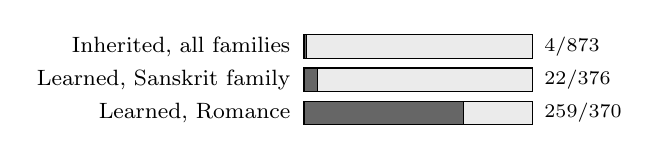
\begin{tikzpicture}[x=1cm,y=1cm,font=\footnotesize]
\node[anchor=east] at (-0.05,1.05) {Inherited, all families};
\draw[fill=black!8] (0,0.90) rectangle (2.9,1.20);
\draw[fill=black!60] (0,0.90) rectangle (0.030,1.20);
\node[anchor=west,font=\scriptsize] at (2.9299999999999997,1.05) {4/873};
\node[anchor=east] at (-0.05,0.63) {Learned, Sanskrit family};
\draw[fill=black!8] (0,0.48) rectangle (2.9,0.78);
\draw[fill=black!60] (0,0.48) rectangle (0.170,0.78);
\node[anchor=west,font=\scriptsize] at (2.9299999999999997,0.63) {22/376};
\node[anchor=east] at (-0.05,0.21) {Learned, Romance};
\draw[fill=black!8] (0,0.06) rectangle (2.9,0.36);
\draw[fill=black!60] (0,0.06) rectangle (2.030,0.36);
\node[anchor=west,font=\scriptsize] at (2.9299999999999997,0.21) {259/370};
\end{tikzpicture}
\caption{Labels that named a different route in October 2024, among sampled pages whose route could be read then. Most Romance learned labels were plain borrowings from Latin two years earlier.}
\label{fig:history}
\end{figure}

\section{A Form-Based Baseline}
\label{sec:baseline}

The audit shows that route claims rarely carry their own citation. If editors mark a word as learned partly because it looks like its etymon, the labels will be predictable from form alone. We test this with deliberately minimal models, under a plan frozen before any feature was computed. \textbf{The target is Wiktionary's label, which is not validated: a score measures how well form predicts the label, not how well it predicts history.}

\paragraph{Setup.} An item is a sense in the audit sample that states exactly one route from the ancestor and gives an ancestor form: 12,778 items in 16 languages. Urdu is left out because its script cannot be compared with Devanagari etyma by our method. Word and etymon are normalised, and Bengali, Gujarati, Gurmukhi and Odia letters are mapped to Devanagari. B1 is a logistic regression on one feature, the normalised edit distance between word and etymon. B3 adds character 1--3-grams of the word and of the etymon. We report macro-F1 for inherited against learned in stratified 5-fold cross-validation; class sizes follow from the sampling design and are roughly equal except in Assamese, Odia and Punjabi (Appendix~\ref{app:denominators}). No parameter was tuned. The standard deviation of B3's macro-F1 over the five folds is at most 0.05 in every language. As a check added after the planned run, we repeated the cross-validation with folds grouped by etymon, so that items sharing an ancestor form stay together: B3 fell by at most 0.013 and rose by at most 0.033 (Armenian). Related words with different ancestor forms can still fall on both sides of a split.

\begin{table}[t]
\centering\small
\setlength{\tabcolsep}{3.5pt}
\begin{tabular}{lrrrrrr}
\toprule
& \multicolumn{2}{c}{\textbf{Macro-F1}} & \multicolumn{3}{c}{\textbf{Mean distance}} & \textbf{Semi as} \\
\textbf{Language} & B1 & B3 & Inh. & Semi & Lrn. & \textbf{learned} \\
\midrule
Assamese & 0.86 & 0.92 & 0.66 & -- & 0.17 & -- \\
Bengali & 0.87 & 0.90 & 0.58 & 0.43 & 0.10 & 14/43 \\
Gujarati & 0.93 & 0.96 & 0.65 & 0.35 & 0.05 & 15/30 \\
Hindi & 0.92 & 0.94 & 0.61 & 0.47 & 0.06 & 22/96 \\
Marathi & 0.87 & 0.90 & 0.58 & -- & 0.05 & -- \\
Odia & 0.89 & 0.91 & 0.63 & -- & 0.11 & -- \\
Punjabi & 0.80 & 0.86 & 0.75 & 0.65 & 0.31 & 12/35 \\
\midrule
Catalan & 0.78 & 0.86 & 0.44 & 0.34 & 0.20 & 32/70 \\
French & 0.86 & 0.91 & 0.52 & 0.39 & 0.22 & 12/25 \\
Galician & 0.77 & 0.87 & 0.46 & 0.48 & 0.24 & 6/26 \\
Italian & 0.70 & 0.75 & 0.41 & 0.35 & 0.25 & 39/58 \\
Portuguese & 0.79 & 0.87 & 0.45 & 0.36 & 0.23 & 74/129 \\
Romanian & 0.81 & 0.87 & 0.46 & -- & 0.20 & -- \\
Spanish & 0.77 & 0.83 & 0.45 & 0.36 & 0.24 & 73/128 \\
\midrule
Greek & 0.57 & 0.62 & 0.10 & -- & 0.04 & -- \\
\midrule
Armenian & 0.48 & 0.59 & 0.12 & 0.21 & 0.11 & 17/31 \\
\bottomrule
\end{tabular}
\caption{Form-based baseline on Wiktionary's labels. Macro-F1 for inherited against learned (majority baseline: 0.33 to 0.42). Mean normalised edit distance to the ancestor form by Wiktionary route. \textit{Semi as learned}: semi-learned items that B3, trained on the other two classes, calls learned; languages with fewer than 20 such items are omitted.}
\label{tab:baseline}
\end{table}

\paragraph{Results.} Table~\ref{tab:baseline} gives the scores. \textbf{For the languages descended from Sanskrit, one number predicts Wiktionary's label}: the distance alone gives macro-F1 between 0.80 and 0.93, and all features give 0.86 to 0.96. For Romance the distance gives 0.70 to 0.86. \textbf{For Greek and Armenian, form barely predicts the label} (0.57 and 0.48 for the distance); in both, inherited and learned words are almost equally close to the ancestor form. \textbf{The semi-learned class lies in between.} In 9 of the 11 languages with at least 20 semi-learned items, its mean distance falls between those of the other two classes, and B3, trained on those two classes, divides it differently by language: the share called learned runs from 23\% to 67\%. The Wilson 95\% interval excludes one half in four languages (Bengali, Hindi and Galician towards inherited, Italian towards learned) and includes it in the other seven. A distance model fitted on the other languages of the same family scores within 0.03 of one fitted on the language itself, except for Punjabi, where it is 0.06 lower (macro-F1 0.74 to 0.93 for Sanskrit, 0.71 to 0.86 for Latin).

\paragraph{Where form and label pull apart.} In a supplementary analysis, planned and frozen after the baseline, we split the items by the distance to the ancestor form. \textit{Congruent} items are inherited and far from it (distance at least 0.5) or learned and close (at most 0.15); \textit{dissociated} items are the reverse. With the same folds, B3 is right on 3,746 of 3,749 congruent items in the seven languages descended from Sanskrit and on 27 of 260 dissociated ones (10\%); for Romance the figures are 98\% and 19\% (52 of 272). Of the 141 Indo-Aryan items that Wiktionary calls inherited although their form is almost the Sanskrit form, B3 is right on two. This is partly by construction: the subsets are defined by a feature of B3, so the split is a diagnostic and not an independent test set. A model that sees only the word, with no etymon and no distance, falls from 87\% to 54\% (Sanskrit) and from 82\% to 74\% (Latin). \textbf{The models reproduce the label where it follows resemblance and fail where it does not.} Dissociated items are few in these two families, about 5\% of the items, so overall scores hide them; in Greek and Armenian they are about a third. They are candidates for validation and not validated cases: each is either a word whose history and form disagree or a labelling error.

\paragraph{Thresholds and a control.} The two thresholds are arbitrary, so we recounted the stored predictions for 15 pairs of them (near from 0.05 to 0.25, far from 0.4 to 0.6), under a plan frozen before the recount. B3 is right on 6\% to 24\% of the dissociated items in the Sanskrit family and on 13\% to 39\% in Romance, and on at least 99.6\% and 96.8\% of the congruent ones; the word-only model stays at 51\% to 61\% and at 69\% to 82\%. No pair brings B3 to one half. Greek and Armenian serve as a control. There form does not predict the label, and B3 does not collapse on the dissociated items: it is right on 144 of 285 (51\%) in Greek and on 134 of 254 (53\%) in Armenian, against 66\% and 65\% of the congruent ones. This is consistent with reading the failure in the other two families as the price of a cue that works there, and not as a property of words that resemble their ancestor.

\section{The Hard Items: A Dictionary and the Missing Link}
\label{sec:link}

\paragraph{The labels that go against resemblance follow a dictionary.} A dissociated item is either a word whose history and form disagree or a labelling error. To tell which, we asked what \citeauthor{turner1966cdial}'s comparative dictionary lists, using the automatic matcher of \S\ref{sec:why}. Among the Indo-Aryan words that are almost the Sanskrit form (distance at most 0.15), Wiktionary calls 141 inherited and 1,571 learned, and B3 cannot tell them apart. Where the etymon heads an article of the dictionary, the article lists a matching form for 57 of 125 of those called inherited (46\%) and for 100 of 1,001 of those called learned (10\%): a difference of 36 points (95\% interval 27 to 45), in the same direction in all seven languages. The first figure equals the rate for ordinary inherited words (48\%). \textbf{Where form misleads the models, Wiktionary's label goes with the dictionary.} This is not independent confirmation, since editors cite this dictionary and the matcher errs at a rate near the learned figure, but it makes labelling error an unlikely account of most of these items. Counts differ below because each analysis needs a further record: 110 of the 141 have a Pali or Prakrit form in the dictionary, and with 84 learned words far from Sanskrit they are the 194 hard items of the model comparison.

\paragraph{The intermediate stage.} An inherited word should carry the changes of the stage it passed through. For the Indo-Aryan items we took the Pali and Prakrit forms that Turner's dictionary lists under the etymon. They are found through the etymon and do not depend on Wiktionary's label. The rule below and its thresholds were frozen before any such form was read; 3,289 of the 4,894 inherited and learned items have such a form. Let $w$ be the word, $a$ the ancestor form and $m$ the intermediate form closest to $w$, all transliterated, with the distance used above. The \textit{link is unchanged} if $m$ is within 0.15 of $a$. Otherwise the word goes \textit{through the link} if it is closer to $m$ than to $a$, and \textit{skips the link} if it is not (Figure~\ref{tab:link}). \textbf{Where the intermediate form changed, the rule alone agrees with Wiktionary}: 967 inherited items go through the link and 517 learned items skip it, 1,484 of 1,864 (80\%), with no training. \textbf{The hard items are those with nothing to change.} For 92 of the 110 near-Sanskrit words that Wiktionary calls inherited (84\%), the Pali or Prakrit form is itself almost the Sanskrit form. These are conservative words: their label can be right, and no comparison of forms can show it. The same holds for 60\% of the learned words that resemble Sanskrit; for the other 40\% the classical argument applies, since the intermediate form changed and the modern word did not. The remaining 18 near-Sanskrit inherited items skip a link that changed, and are candidates for a wrong or a semi-learned label.

\begin{figure}[t]
\centering
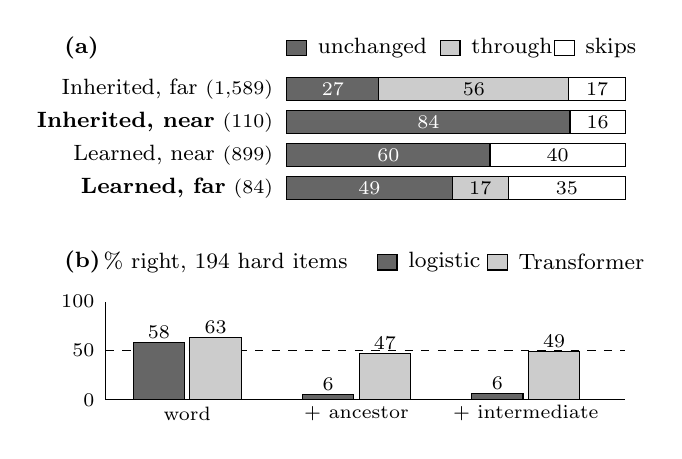
\begin{tikzpicture}[x=1cm,y=1cm,font=\footnotesize]
\node[anchor=east] at (-0.05,3.20) {Inherited, far {\scriptsize(1,589)}};
\draw[fill=black!60] (0.000,3.05) rectangle (1.169,3.35);
\node[text=white,font=\scriptsize] at (0.585,3.20) {27};
\draw[fill=black!20] (1.169,3.05) rectangle (3.583,3.35);
\node[text=black,font=\scriptsize] at (2.376,3.20) {56};
\draw[fill=white] (3.583,3.05) rectangle (4.300,3.35);
\node[text=black,font=\scriptsize] at (3.941,3.20) {17};
\node[anchor=east] at (-0.05,2.78) {\textbf{Inherited, near} {\scriptsize(110)}};
\draw[fill=black!60] (0.000,2.63) rectangle (3.596,2.93);
\node[text=white,font=\scriptsize] at (1.798,2.78) {84};
\draw[fill=white] (3.596,2.63) rectangle (4.300,2.93);
\node[text=black,font=\scriptsize] at (3.948,2.78) {16};
\node[anchor=east] at (-0.05,2.36) {Learned, near {\scriptsize(899)}};
\draw[fill=black!60] (0.000,2.21) rectangle (2.578,2.51);
\node[text=white,font=\scriptsize] at (1.289,2.36) {60};
\draw[fill=white] (2.583,2.21) rectangle (4.300,2.51);
\node[text=black,font=\scriptsize] at (3.441,2.36) {40};
\node[anchor=east] at (-0.05,1.94) {\textbf{Learned, far} {\scriptsize(84)}};
\draw[fill=black!60] (0.000,1.79) rectangle (2.099,2.09);
\node[text=white,font=\scriptsize] at (1.049,1.94) {49};
\draw[fill=black!20] (2.099,1.79) rectangle (2.815,2.09);
\node[text=black,font=\scriptsize] at (2.457,1.94) {17};
\draw[fill=white] (2.815,1.79) rectangle (4.300,2.09);
\node[text=black,font=\scriptsize] at (3.558,1.94) {35};
\draw[fill=black!60] (0,3.62) rectangle (0.25,3.82); \node[anchor=west] at (0.27,3.72) {unchanged};
\draw[fill=black!20] (1.95,3.62) rectangle (2.2,3.82); \node[anchor=west] at (2.22,3.72) {through};
\draw[fill=white] (3.4,3.62) rectangle (3.65,3.82); \node[anchor=west] at (3.67,3.72) {skips};
\node[anchor=west,font=\footnotesize\bfseries] at (-2.95,3.72) {(a)};
\node[anchor=west,font=\footnotesize\bfseries] at (-2.95,1.0) {(b)};
\node[anchor=west] at (-2.45,1.0) {\% right, 194 hard items};
\draw[fill=black!60] (1.15,0.9) rectangle (1.4,1.1); \node[anchor=west] at (1.42,1.0) {logistic};
\draw[fill=black!20] (2.55,0.9) rectangle (2.8,1.1); \node[anchor=west] at (2.82,1.0) {Transformer};
\draw (-2.3,-0.75) -- (4.3,-0.75); \draw (-2.3,-0.75) -- (-2.3,0.50);
\node[anchor=east,font=\scriptsize] at (-2.32,-0.75) {0};
\node[anchor=east,font=\scriptsize] at (-2.32,-0.12) {50};
\node[anchor=east,font=\scriptsize] at (-2.32,0.50) {100};
\draw[dashed] (-2.3,-0.125) -- (4.3,-0.125);
\draw[fill=black!60] (-1.95,-0.75) rectangle (-1.30,-0.022);
\node[font=\scriptsize] at (-1.625,0.108) {58};
\draw[fill=black!20] (-1.23,-0.75) rectangle (-0.58,0.042);
\node[font=\scriptsize] at (-0.905,0.172) {63};
\node[font=\scriptsize] at (-1.265,-0.92) {word};
\draw[fill=black!60] (0.20,-0.75) rectangle (0.85,-0.679);
\node[font=\scriptsize] at (0.525,-0.549) {6};
\draw[fill=black!20] (0.92,-0.75) rectangle (1.57,-0.164);
\node[font=\scriptsize] at (1.245,-0.034) {47};
\node[font=\scriptsize] at (0.885,-0.92) {+ ancestor};
\draw[fill=black!60] (2.35,-0.75) rectangle (3.00,-0.672);
\node[font=\scriptsize] at (2.675,-0.542) {6};
\draw[fill=black!20] (3.07,-0.75) rectangle (3.72,-0.137);
\node[font=\scriptsize] at (3.395,-0.007) {49};
\node[font=\scriptsize] at (3.035,-0.92) {+ intermediate};
\end{tikzpicture}
\caption{The intermediate stage, seven Indo-Aryan languages. (a) Items with a Pali or Prakrit form in Turner's dictionary, by Wiktionary label and distance to the Sanskrit form (near and far as in Figure~\ref{fig:grid}; $n$ in brackets; dissociated rows in bold). Percentages: intermediate form unchanged from Sanskrit, word closer to the intermediate form (through), word not showing its change (skips). (b) Accuracy on the dissociated items by model input (the word; with the ancestor form; with the intermediate form as well), both models on the same pooled folds (Appendix~\ref{app:further}); the dashed line is 50\%.}
\label{tab:link}
\end{figure}

\paragraph{The link does not repair the model.} We compared three inputs on the 3,289 linked items, with folds grouped by etymon: the word alone, the word with the ancestor form (B3), and both with the intermediate form (Figure~\ref{tab:link}b). For the linear model macro-F1 is 0.78, 0.90 and 0.90, and it is right on 113 (58\%), 11 (6\%) and 12 (6\%) of the 194 dissociated items. \textbf{The ancestor form buys the overall score at the cost of the hard items, and the intermediate form restores nothing.} Two neural models on the same folds agree. A character Transformer trained from random initialisation scores 0.78, 0.86 and 0.86 and is right on 63\%, 47\% and 49\% of the hard items; a pretrained character model, CANINE-S \citep{clark2022canine}, scores 0.76, 0.84 and 0.85 and is right on 59\%, 56\% and 51\%. Neither collapses as the linear model does, but with the forms both are at chance and neither beats the word alone. \textbf{In none of the three models does the intermediate form help}: on these items the link carries no change to detect. Settings, intervals, the counts with folds made per language (120, 15 and 23 for the linear model), abstention and a finer, segment-based distance are in Appendix~\ref{app:further}.

\paragraph{What does help, and how far.} If form is a shortcut, a model can be kept from it. We gave B3 three things that are not form: training weights that balance route against distance band; the meaning of the word, as the words of its definition; and, for the Sanskrit family, the matcher's record of Turner's dictionary. In the Sanskrit family, accuracy on the 260 dissociated items rises from 10\% to 41\% with the weights, to 25\% with the dictionary record, and to 53\% with all three (95\% interval 47--59), for a macro-F1 of 0.890 against 0.912. In Romance the weights raise it from 19\% to 44\%. Meaning added alone changes little. \textbf{The collapse on the hard items is avoidable; the ceiling is not}: no condition passes the model that sees the word alone (54\% and 74\%). A higher score here is closer agreement with Wiktionary, not historical accuracy (Appendix~\ref{app:further}).

\paragraph{A large language model.} A large language model might simply know the record. Two passes of one model (Claude Sonnet 4.6, under two instruction sets) labelled the hard Indo-Aryan items and matched controls from the word alone. Where a pass chose inherited or learned, it agrees with Wiktionary on 93\% and 94\% of the controls, on 85\% and 82\% of the learned words far from Sanskrit, and on 34\% and 45\% of the near-Sanskrit words called inherited (38 of 113; 49 of 110). \textbf{On the words that resemble their ancestor, this model follows form as well.} The two passes agree on 89\% of rows ($\kappa=0.82$); that is the consistency of one model, not inter-annotator agreement. Most of its labels cite no source, and its blindness to Wiktionary is not guaranteed (Appendix~\ref{app:further}).

\paragraph{Expert judgements.} Two open sources give specialists' loan judgements for basic meanings. In the Romanian vocabulary of the World Loanword Database \citep{schulte2009romanian}, the specialist considers 651 of the 684 inherited-category titles found there not borrowed (95.2\%; 95\% interval 93.3 to 96.5). In the IE-CoR database \citep{heggarty2024iecor}, which includes thirteen of our languages from all four families, 277 of 291 inherited-category titles are not loans (95.2\%; 92.1 to 97.1). Both hold few learned-category words (28 and 21). \textbf{On the dissociated items the specialists side with Wiktionary.} IE-CoR judges 48 of them, 46 of which are near-ancestor words called inherited (32 Greek or Armenian): it agrees with Wiktionary on 45 (94\%; 83 to 98), and B3 agrees with it on 22. The Romanian source agrees with Wiktionary on all six that it judges, B3 on one. These are few words, judged by one specialist or one team; this is not a two-annotator validation, and it says little about learned labels.

\paragraph{Reading these results.} High scores on these labels do not show that the labels are right, and low scores on the hard items do not show that they are wrong. For most words that resemble the ancestor, the intermediate stage resembles it too, so the route is a matter of record (attestation, dating, a lexicographer's judgement) and not of form. A classifier evaluated on Wiktionary's labels should report its score on the dissociated items separately, and cannot be expected to recover more than the sources behind the labels supply. Whether those sources can be consulted independently is the subject of the next section, for Hindi and Bengali.

\section{Can Dictionaries Decide the Route?}
\label{sec:why}

If the route is a matter of record, the record should be open to consultation. We tested this on 48 Hindi and Bengali lemmas (58 senses), chosen in strata by a keyed hash under rules frozen before any page was retrieved, in four dictionaries: \citet{platts1884} and \citet{dasa1975sabdasagara} for Hindi, \citet{dasa1937bangala} for Bengali, and \citet{turner1966cdial} for both. Phonological shape never decides a label: a route is assigned only where a source states it or where it follows from a convention documented in the source's front matter. The lookups were automated: a language model (Claude) ran the dictionary searches and read the entries from a blind sheet that showed only the lemma and a gloss, and the labels were frozen before the Wiktionary side was opened. The labels are model-extracted and are not gold labels. One author compared the 23 pilot rows with the dictionary entries, and all matched; the 111 rows of the second round are unchecked. Appendix~\ref{sec:method} gives the method, the rules and the tables. We report raw counts, which estimate no rate.

\paragraph{Results.} A route could be assigned to 26 of the 58 senses, 17 of 28 for Hindi and 9 of 30 for Bengali; 22 were found in a dictionary that states no route, and 10 in no dictionary. Where a route was assigned, it agrees with Wiktionary's templates on 22 senses and disagrees on 3. \textbf{No inherited or learned label rests on an explicit statement in a source}: all 5 explicit labels are external loans. Of the 12 senses that Wiktionary calls semi-learned, none was recovered, and of the 9 Bengali learned ones, none. Three properties of the sources account for this. None has a mark for a partly adapted loan. The Bengali dictionary gives a Sanskrit analysis for words that look inherited and for words that look learned alike, and for Hindi all 6 learned labels rest on one marker in a dictionary of 1884. And an unmarked listing in Turner's dictionary, on which 11 of the 13 inherited labels of the second round rest, is weaker evidence than its convention suggests, since he lists modern forms identical to the Sanskrit word with no loan mark.


\paragraph{The same rule at scale.} We applied the rule by program to the baseline items of seven Indo-Aryan languages, through a machine-readable copy of Turner's dictionary \citep{arora2023jambu}. The copy carries no licence, so we used it for analysis only and release nothing from it. The plan was frozen before the file was read, and the matcher was first compared with our hand records: it agreed in 31 of 38 rows, missing 4 listed forms and accepting 3 near variants that the hand record had rejected. Among matched items, a listed form matches the Wiktionary word for 49\% of the inherited ones and for 9.1\% of the learned ones (130 of 1,435). \textbf{The second figure is of the same size as the matcher's false-positive rate, so it gives 130 candidates for a manual check and not a leak rate.}

\section{Discussion}

The dictionary method works where it is least needed. Inherited words that Turner lists and plain foreign loans are recovered, and these are also the cases in which Wiktionary and the dictionaries agree. The method fails on the boundary between learned and semi-learned words, and for Bengali on the boundary between inherited and learned words, because the sources have no means to express it.

A different kind of source could change this: a post hoc, non-blind search of a historical grammar found the semi-learned label stated explicitly for 2 of the 6 Bengali cases (Appendix~\ref{app:further}).

For work that trains or evaluates on Wiktionary's route labels we suggest three practices. (i) Report the score on the items whose label goes against resemblance beside the overall score, which hides them, and treat that split as a diagnostic; weighting the training items by route and distance band removes most of the collapse there at a small cost overall. (ii) Keep agreement with the dictionary's labels apart from agreement with independent evidence, and say which is reported. (iii) Read routes per sense from the etymology, since up to 17.5\% of titles carry more than one, and do not expect the semi-learned class (at most 129 pages in any language) or, in our sample, the Bengali learned labels to be checkable against these dictionaries.

\section*{Limitations}

\begin{itemize}
\item \textbf{The sample is small and not random.} There are 48 lemmas in strata chosen to over-sample hard cases. The counts describe this sample only.
\item \textbf{The dictionary labels are model-extracted and only partly verified} (\S\ref{sec:extraction}). There is no second annotator and no inter-annotator agreement. The human check covers the 23 pilot rows (no discrepancy); an error in the 111 rows of round~2 would not have been caught.
\item \textbf{Some absences may be search failures.} The Bengali dictionary uses older spellings, and 8 of 30 Bengali senses were found in no source.
\item \textbf{The Turner head-word was often the extractor's choice}, taken from the language dictionary's etymology where it gave one. A wrong choice produces a false ``not listed''. Turner was not queried for 5 senses that are plain foreign loans.
\item \textbf{Judgement was needed} to decide whether a near variant of a form counts as listed. We did not count near variants; a looser rule would move 2 senses from \lbl{unk} to inherited.
\item \textbf{The two rounds used different protocol versions.} The 12 pilot senses were labelled under v1.0, before senses were separated by rule, and were not relabelled. One pilot row was reclassified from ``disagree'' to ``candidate unspecified'' when the template-based candidate was applied.
\item \textbf{The expert checks are small and concern basic vocabulary}: one specialist for Romanian and one team for thirteen languages, matched to our items by spelling, with few learned words and only 48 and 6 dissociated items; neither source separates learned from semi-learned borrowing.
\item \textbf{The supplementary analyses were planned after the main ones.} The dissociated subset is defined by a model feature, so the low score on it is partly by construction, and no recount of thresholds removes that; its items are unvalidated, and the program reading of Turner's dictionary agreed with our hand records in 31 of 38 rows only.
\item \textbf{The analysis of the intermediate stage is orthographic and partial.} It compares transliterated spellings, not transcriptions; the finer distance that we also report rests on a feature table of our own, and no such comparison was made for Romance. Pali and Prakrit are not the direct ancestors of each modern language. A Pali or Prakrit form was found for 67\% of the items. The thresholds were fixed in advance and are arbitrary. The links that Wiktionary records are not independent of its labels, and the agreement of the hard items with Turner's dictionary is not independent either, since editors cite that dictionary.
\item \textbf{Two defects were found late and corrected.} In a first run our template reader took a transliteration parameter for the ancestor form in 21 items, and four analyses attached items to their subset by spelling. We corrected both and reran the baseline and every analysis built on it; all figures here are from the corrected run (the first run gave 14\% where we now report 10\%). Two things were not redone: the language-model check, in which 20 of 4,360 prompts showed the misread form, and the blind annotation sheets.
\item \textbf{The baseline predicts unvalidated labels.} Its etymon comes from the same entry as the label, senses with several routes are left out, classes are balanced by design, and nothing was tuned or tested for significance.
\item \textbf{Most Romance learned labels in the history sample were set by one automated account in September 2026.} We do not know its rule; if it relabelled every borrowing from Latin, the Romance learned class is that class under a new name. The history sample is the first 60 pages of each category.
\item \textbf{The language-model passes are not annotation} (Appendix~\ref{app:further}): one model, mostly labelling from form, with unverified references and no guarantee of blindness.
\item \textbf{The audit validates no label.} It counts what Wiktionary records. Its inline-citation measure misses sources listed only at the foot of an entry, and its template reader counts an etymology written as plain text as stating no route. Its 17 pairs are related and are not independent tests.
\item \textbf{The check of the historical grammar is exploratory.} It was made after the Wiktionary labels were known, on a scanned text.
\item \textbf{The sources are old and few.} The Hindi learned labels depend on a dictionary of 1884. We did not read the front matter of the \textit{Hind\=\i{} \'sabdas\=agara}, so it contributed no route, and we did not consult the modern Hindi dictionary that Wiktionary cites most often.
\end{itemize}

\section*{Ethical Considerations}

One dictionary is in the public domain, and we treat the other three as in copyright. We consulted them through a public library interface with single queries at least two seconds apart, and we stored entry references and paraphrases only. Wiktionary text is used under its licence, with page revisions recorded; the audit read 13,128 pages through the public interface in serial requests. No human participants were involved. A language model was used for dictionary lookups and label extraction (\S\ref{sec:extraction}), to fill the sheets of the two passes reported in \S\ref{sec:link}, to run the analysis scripts, and to assist with drafting. The authors directed the research and are responsible for the paper's content.

\bibliography{refs}

\appendix

\section{Protocol Records}
\label{app:records}

The selection rules, both protocol versions, the blind sheets, the frozen label files and the source checks are kept with SHA-256 hashes in a dated decision log. We intend to release what is derived from Wiktionary (the item lists with revision identifiers, the subsets, the baseline predictions and the recorded intermediate forms), the scripts and the frozen plans, and, for the dictionary study, entry references and our paraphrases. No dictionary text is released, and nothing from the machine-readable copy of Turner's dictionary.

\begin{table}[h]
\centering\small
\begin{tabular}{p{0.60\columnwidth}p{0.28\columnwidth}}
\toprule
\textbf{Observation} & \textbf{Route} \\
\midrule
Turner lists the form, with no loan mark & inherited \\
Turner marks the form as a loanword & as stated \\
Turner has the etymon, but no form for the language & not stated \\
Platts marks the word S & learned \\
Platts marks it H and cites a Prakrit form & inherited \\
Platts marks it H, Sanskrit form only & not stated \\
Platts marks it P, A or T & external \\
J.~D\=asa cites a Pali or Prakrit form & inherited \\
J.~D\=asa cites only Sanskrit & not stated \\
J.~D\=asa cites a non-Indo-Aryan source & external \\
\bottomrule
\end{tabular}
\caption{Label rules of protocol v1.1 (abridged). All inherited and learned routes in this table have structural strength.}
\label{tab:rules}
\end{table}

\section{The Dictionary Study in Full}
\label{sec:method}

\subsection{Items}

We selected 48 lemmas from English Wiktionary, 24 for Hindi and 24 for Bengali. The selection rules were frozen, with a recorded SHA-256 hash, before any category member list was retrieved. Each language has seven strata defined by category membership: three lemmas that belong to two or more of the learned, semi-learned and inherited categories (the \textit{overlap} stratum), six from each of those three categories, and one borrowing each from Persian, Arabic and English. Within a stratum, lemmas are ordered by a keyed hash of the title, and the first $n$ are taken. Selection uses only the page title and its category membership. The revision of each page was recorded.

The unit of analysis is the \textbf{sense}: a lemma with several Etymology sections on Wiktionary gives one row per section. The 48 lemmas give 58 sense rows, 28 for Hindi and 30 for Bengali. One of the 58 is a homograph found in a dictionary and absent from Wiktionary; it has no Wiktionary candidate.

\subsection{Sources}

All entries were consulted through the search interface of the Digital South Asia Library. The queries were issued one at a time, at least two seconds apart.
\begin{itemize}
\item \textbf{\citet{platts1884}}, for Hindi. Each headword carries a letter for its language of origin: S for Sanskrit, H for Hindi, P, A and T for Persian, Arabic and Turkish.
\item \textbf{\citet{turner1966cdial}}, for both languages. Each article has an Old Indo-Aryan head-word followed by its Middle and New Indo-Aryan descendants. The front matter defines a sign and an abbreviation for loanwords.
\item \textbf{\citet{dasa1937bangala}}, for Bengali. The entries cite Sanskrit, Pali, Prakrit and foreign source forms.
\item \textbf{\citet{dasa1975sabdasagara}}, for Hindi, as a lookup source only. We did not read its front matter, so its entries assert no route under our rules.
\end{itemize}
We read the conventions of the first three dictionaries from their front matter before relying on them, and we store entry references and paraphrases only (Appendix~\ref{app:further}).

\subsection{Labels and rules}

Each sense receives one label: inherited (\lbl{inh}), learned (\lbl{lrn}), semi-learned (\lbl{semi}), external loan (\lbl{ext}), disputed between sources (\lbl{dis}), found with no route stated (\lbl{unk}), or found in no source (\lbl{nsf}). Table~\ref{tab:rules} (Appendix) gives the rules that connect a dictionary observation to a route. Phonological shape alone never decides a label. \lbl{semi} is assigned only on an explicit statement, and we expected it to be unrecoverable because no source has a marker for it. Each label also carries an evidence strength: \textit{explicit} if the source states the route, \textit{structural} if the route follows from a documented convention of the source, and \textit{none}.


\subsection{Blinding and freezing}

The extractor worked from a blind sheet that showed only the item identifier, the language, the lemma and a short gloss. A script built the sheet from the stored Wiktionary pages and printed nothing else, so the etymology text, the templates and the categories stayed unseen. After all lookups the labels were frozen with a SHA-256 hash, and only then was the Wiktionary side opened.

The Wiktionary \textbf{candidate} for a sense is read by a script from the etymology templates in that sense's own Etymology section.

The work ran in two rounds, a pilot of 10 lemmas under protocol v1.0 and 38 lemmas under v1.1, which was frozen before any of them was seen (Appendix~\ref{app:further}).

\subsection{Extraction}
\label{sec:extraction}

The rules above were frozen before any lookup. The lookups were then automated: a language model (Claude) ran the dictionary searches and read the entries under those rules. Each of the 134 source-check rows records the query, the entry reference, a paraphrase of the evidence and the route asserted; 5 rows record that a source was not queried. The resulting labels are model-extracted. They are not gold labels, and we report no inter-annotator agreement. \textbf{Verification.} One author compared the 23 pilot rows with the dictionary entries, for entry reference and paraphrase; all matched. These are all the pilot rows, not a random sample. The 111 rows of round~2 are unchecked.

\subsection{Results}

\begin{table}[h]
\centering\small
\begin{tabular}{lrrr}
\toprule
\textbf{Label} & \textbf{Hindi} & \textbf{Bengali} & \textbf{Total} \\
\midrule
Inherited & 8 & 7 & 15 \\
Learned & 6 & 0 & 6 \\
External loan & 3 & 2 & 5 \\
Semi-learned, disputed & 0 & 0 & 0 \\
\midrule
Found, no route stated & 9 & 13 & 22 \\
Found in no source & 2 & 8 & 10 \\
\midrule
Total & 28 & 30 & 58 \\
\bottomrule
\end{tabular}
\caption{Source-based labels for the 58 sense rows (pilot and round~2 together).}
\label{tab:labels}
\end{table}

\paragraph{Coverage.} Table~\ref{tab:labels} gives the source-based labels. A route was assigned to 26 of the 58 senses: 17 of 28 for Hindi and 9 of 30 for Bengali. Of the remaining 32, 22 were found in a dictionary that states no route, and 10 were found in no dictionary. By evidence strength, 5 labels are explicit, 21 are structural and 32 senses have none; for the 12 pilot senses the strength was re-read after the dictionary conventions had been verified, with no change of label. All 5 explicit labels are external loans. \textbf{No inherited or learned label rests on an explicit statement in a source.}

\begin{table}[h]
\centering\small
\begin{tabular}{lrrrrr}
\toprule
\textbf{Wiktionary} & \textbf{$n$} & \textbf{Same} & \textbf{Other} & \textbf{\lbl{unk}} & \textbf{\lbl{nsf}} \\
\midrule
Inherited & 16 & 12 & 0 & 3 & 1 \\
Learned & 19 & 5 & 1 & 10 & 3 \\
Semi-learned & 12 & 0 & 2 & 7 & 3 \\
External & 8 & 5 & 0 & 0 & 3 \\
Other & 3 & -- & 1 & 2 & 0 \\
\bottomrule
\end{tabular}
\caption{Source-based outcome by Wiktionary candidate. \textit{Same}: the sources assign the candidate's label. \textit{Other}: they assign a different label. \textit{Other} candidates are unspecified, unknown or absent.}
\label{tab:recover}
\end{table}

\paragraph{Recoverability by category.} Table~\ref{tab:recover} splits the senses by Wiktionary candidate. The sources assign the same label to 12 of 16 inherited candidates and to 5 of 8 external candidates. They assign it to 5 of 19 learned candidates, and all 5 are Hindi; of the 9 Bengali learned candidates, none was recovered. Of the 12 semi-learned candidates, none was recovered: 2 were labelled inherited by the sources, 7 were found with no route, and 3 were not found.

\paragraph{Agreement.} On the 26 senses with a source-based route, the sources and the Wiktionary candidate agree on 22 and disagree on 3; for the remaining one the candidate is unspecified, because the page carries both a borrowing and an inheritance template. The three disagreements are Hindi \textit{b\=a\~ncn\=a} \gl{to read} and \textit{am\=avas} \gl{new moon}, which the sources label inherited and Wiktionary semi-learned, and Bengali \textit{bh\=al} \gl{forehead}, which the sources label inherited and Wiktionary learned.

\textbf{This agreement is not fully independent.} We checked whether the Hindi or Bengali entry on Wiktionary cites the dictionary on which our label rests. Of the 22 agreeing senses, 4 inherited ones cite the same Turner article that we used, and 3 of the 5 learned ones are in entries that cite Platts. The other 15 cite neither, although an entry can draw on a source without citing it. Of the 28 Hindi senses, 20 are in entries that cite a modern Hindi dictionary that we did not consult.

\subsection{Why the boundary is not recoverable}

\paragraph{No source marks semi-learned words.} None of the three dictionaries whose conventions we read has a label or a sign for a partly adapted Sanskrit loan; we did not read the conventions of the fourth. J.~D\=asa's list of abbreviations has a label for a ``Bengali Prakritic form'', but it describes the form and does not state a route. The category cannot be recovered by this method.

\paragraph{Bengali has no equivalent of Platts' S.} In the entries that we consulted, J.~D\=asa gives a Sanskrit analysis for words that look inherited and for words that look learned alike. A reader cannot tell from the entry whether the Sanskrit form is an ancestor or a donor. For Hindi, all 6 learned labels rest on the S marker of \citet{platts1884} alone.

\paragraph{The inherited rule is leaky.} The front matter of \citet{turner1966cdial} says that the forms listed in an article are descendants of the head-word, and it defines marks for loanwords. It does not say that every loan is marked. In the entries that we consulted, Turner lists modern forms that are identical to the Sanskrit word and carry no loan mark: Hindi \textit{h\=ani} \gl{loss}, Bengali \textit{kamal\=a} \gl{orange} and Bengali \textit{bh\=al} \gl{forehead}. An unmarked listing is therefore weaker evidence of inheritance than the convention suggests. Of the 13 inherited labels in round~2, 11 use this rule, and 10 of those have no other support.

\section{Further Checks}
\label{app:further}

\paragraph{Two language models: no conclusion.} We put the dissociated items and matched controls to two open-weight language models run locally (Gemma~3, 4 and 12 billion parameters; fixed prompts, temperature 0; 4,360 answers each), under plans frozen in advance. Both answered ``inherited'' whatever the word, the smaller about four times in five and the larger in 97\% of answers, with balanced scores of 0.50 to 0.60. Both runs are null results and support no claim here.

\paragraph{Citation and predictability.} Greek has both the most inline citations and low predictability. We checked whether the two are linked within languages. In the eight languages with at least 30 cited and 30 uncited items, B3 is slightly more accurate on cited items in seven, with overlapping intervals, and the comparison is confounded by route. We find no support for a link and do not claim one.

\paragraph{One correction after the first run.} The first run reported that up to 28\% of pages in an inherited category had no supporting template. Inspection showed a defect in our template reader, which missed the nested form of a newer etymology template. We corrected the reader, extended a hand-worked test fixture to cover that form, and reran the audit. We report the corrected figures and keep the first run on file.

\paragraph{The hard-boundary stratum was mostly homographs.} The overlap stratum was meant to hold words whose route is contested. Of its 6 lemmas, 5 are pairs of unrelated words with one spelling, one inherited and one learned according to Wiktionary's templates. The sixth is in the inherited category only because a template for derived terms adds the category, although the page's etymology template is a learned borrowing. None of the 6 is a single word with a contested route. The audit shows that such pages are rare (Table~\ref{tab:audit}), so this stratum selected an unusual kind of page and did not sample hard boundary cases.

\paragraph{A post hoc check of a historical grammar.} After the study was complete, we searched the text of \citet{chatterji1926} for the 6 Bengali senses that Wiktionary calls semi-learned. \textbf{This check was not blind, it followed no frozen rule, and it used a scanned text; it adds no labels to our counts.} Chatterji uses the abbreviations \textit{ts.}, \textit{sts.} and \textit{tbh.} for tatsama, semi-tatsama and tadbhava words. He calls \textit{j\=ait} \gl{caste} and \textit{jochn\=a} \gl{moonlight} semi-tatsama explicitly (vol.~1, pp.~308 and 470). Two more, \textit{soy\=ad} \gl{taste} and \textit{soy\=ami} \gl{husband}, appear in a list that opens with that label (p.~534), and 2 were not found. The distinction that the dictionaries cannot express is therefore stated in the scholarly literature for some words. A grammar cites words as examples and has no entry for every word, so its coverage of a random sample is unknown. The passages were read in the machine-recognised text of the scan and were not compared with the page images.

\paragraph{A neural model on the three inputs.} To see whether the result depends on the linear model, we trained a character Transformer (3 layers, width 128, from random initialisation, no pretrained model, nothing tuned, 5 seeds averaged) on the same 3,289 linked items, with the seven languages pooled and folds grouped by etymon over all of them; the plan was frozen before any training. The logistic models were rerun on these folds for reference. Macro-F1 for the word alone, with the ancestor form, and with the intermediate form as well is 0.78, 0.90 and 0.90 for the logistic models and 0.78, 0.86 and 0.86 for the Transformer. On the 194 dissociated items the logistic models are right on 113, 11 and 12, and the Transformer on 123, 91 and 95 (47\% and 49\%; intervals 40--54\% and 42--56\%). The Transformer is therefore near chance on these items where the linear model is far below it, and it pays for this on the congruent items (93\% against nearly 100\%). \textbf{In neither model does the intermediate form help, and in neither does a model that sees the ancestor form beat the one that sees the word alone on these items.} When the Transformer's least confident predictions are set aside, dissociated items are dropped more often than others (at 50\% coverage 38 of 194 are kept) but the ones kept are still at chance (18 of 38). An earlier planned test that added only the two link distances to the linear model gave 32 against 34 of 194. On the 110 dissociated inherited items the linear models with the ancestor form are right on one without the intermediate form and on four with it (per-language folds). Neither finding depends on the coarse transliteration: with a segment-based distance that keeps vowel length, retroflexion, sibilants and aspiration (frozen before it was computed), 92 of the 110 hard inherited items again have an unchanged link, or 74 with the strictest costing, and the models are right on 37 and 35 of 194.

\paragraph{A pretrained model on the three inputs.} Under a plan frozen before any pretrained model was loaded, we fine-tuned CANINE-S \citep{clark2022canine} on the items and folds of the Transformer above (all weights, learning rate $3\times10^{-5}$, 8 epochs, batch 32, 3 seeds averaged, nothing tuned), on a hosted GPU. The plan names 3,276 items, the count before the correction described in the Limitations; the run used the corrected 3,289. Macro-F1 for the word alone, with the ancestor form, and with the intermediate form as well is 0.76, 0.84 and 0.85 (single seeds 0.74 to 0.84). On the 194 dissociated items the three are right on 115 (59\%; 52--66), 109 (56\%; 49--63) and 98 (51\%; 44--57), and on 81\%, 91\% and 91\% of the congruent ones. By the readings fixed in the plan, the intermediate form does not help a pretrained model, and with the forms it does not beat the word-only models. Within the dissociated items it is right on 61 of the 84 learned words far from Sanskrit with the ancestor form (49 without) and on 48 of the 110 inherited words near it (66 without); the intervals overlap in the first case. At 50\% coverage 48 dissociated items are kept and 30 are right. The linear models were fitted again in that environment as a reference and give 115, 9 and 9 of 194 there, against 113, 11 and 12 on our machine; we take the difference to come from library versions and report the latter in the main text. These figures are from the run's printed summary.

\paragraph{Details of the hard-item analyses.} Each analysis of \S\ref{sec:link} followed a plan frozen before it was computed. \textit{Dictionary.} Over all matched items, whatever their form, the matcher gives 49\% and 9.1\% (\S\ref{sec:why}); for ordinary inherited words far from the Sanskrit form the rate is 976 of 2,027, and for words far from it that Wiktionary calls learned, 5 of 97. Of the 141 near-Sanskrit words called inherited, 125 have an etymon that heads an article. \textit{Expert sources.} Of the 28 learned-category words found in the Romanian source, 19 are borrowed with Latin as a donor. \textit{What does help.} On the baseline's items and folds, in the Sanskrit family the weights give 106 of 260 dissociated items (41\%; 35--47), the dictionary flags 66 (25\%; 20--31) with macro-F1 0.919 against 0.912 (mean over languages), meaning 30 (12\%), and all three 138 (53\%; 47--59), with 93\% of congruent items right. In Romance the weights give 120 of 272 (44\%; 38--50) for 0.025 of macro-F1, and meaning 67 (25\%; its interval overlaps B3's). A model that sees only the definition is right on 89 of the 141 near-Sanskrit words called inherited, which are often basic vocabulary. The flags come from the dictionary that the editors cite.

\paragraph{The two passes of a large language model.} All 22 blind sheets of our first annotation kit were filled by a language model (Claude Sonnet 4.6) in two passes under two instruction sets; the sheets show the word only. \textbf{These are not expert annotation, and agreement between the passes is not inter-annotator agreement.} In the first pass, 728 of 879 rows give no source beyond ``linguistic analysis'': the label was assigned from the form of the word. Where both passes cite an entry of Turner's dictionary for one word, the entry numbers differ in 58 of 79 cases, so the references are unverified. The session that filled the Hindi sheet also regenerated its answer key, so blindness to Wiktionary's label is not guaranteed, and the model may have seen Wiktionary in training. Under a plan frozen before the comparison, we kept the rows of the seven Indo-Aryan dissociation sheets that are still controls or dissociated items in the corrected baseline (272 and 251 rows). Among rows labelled inherited or learned, the passes agree with Wiktionary on 209 of 225 and 214 of 227 controls; on 126 of 216 and 138 of 219 dissociated items (58\% and 63\%); within these, on 88 of 103 and 89 of 109 learned words far from Sanskrit, and on 38 of 113 and 49 of 110 near-Sanskrit words called inherited. The passes agree with each other on 89\% of 466 rows (Hindi left out; $\kappa=0.82$). The general sheets for Hindi, Bengali, French and Romanian are not analysed here.

\paragraph{The history of the labels.} For the first 60 pages of each category (3,250 sample rows, 2,575 pages) we read the last revision before 11 October 2024 and before 11 October 2021 with the same template reader, under a plan frozen before any past revision was retrieved. \textbf{Inherited labels are stable}: of 873 that stated a route from the ancestor in 2024, 4 named a different one. \textbf{Learned labels in Romance are recent}: of 370 that stated a route in 2024, 259 (70\%; 65--74) named a different one, and 258 of these were marked as plain borrowings from Latin; in 2021 the figure is 171 of 178. For the languages descended from Sanskrit it is 22 of 376 (6\%) in 2024 and 50 of 126 in 2021, again mostly plain borrowings. The learned label in these languages is thus largely a later relabelling of words that were already marked as borrowed from the ancestor. Changes between inherited and learned are rare: 5 pages that are now learned were inherited in 2024, over all four families. In a further analysis frozen before any revision list was requested, we looked for the first revision after the 2024 snapshot in which each changed page states the learned route, and recorded its month and an unlinkable pseudonym of the account. For Romance, 252 of the 259 changes were located: 241 fall in September 2026 and 240 were made by one account in the bot group. \textbf{The learned label on these Romance pages is thus largely one automated relabelling, made a month before we sampled, of words already marked as borrowed from Latin.} We do not know the rule that the account applied, and we did not ask its operator. A score on the Romance learned labels is therefore best read as inherited against borrowed from Latin. For the languages descended from Sanskrit the 22 changes were all located and are spread: ten accounts over fifteen months, at most three in a month, one by a bot. In a check added after the plan, the revision histories show that the learned-borrowing template was created in August 2015 and its short form in February 2016, so the late change in Romance is not the arrival of the template: it had been available for nine years while these words were marked as plain borrowings. Labels on dissociated items were not changed more often than labels on congruent items (8 of 141 against 87 of 819 in 2024), so we make no claim that editors were less certain of them. A stable label is not a correct label.

\paragraph{The links that Wiktionary records.} Inherited entries often name an intermediate form themselves. In the Latin family 1,006 of 2,778 inherited items do (Old French, Old Spanish, Old Galician-Portuguese or Old Catalan). Of these, 917 (91\%) go through that link and 35 skip it; of the 47 dissociated ones, 42 have an unchanged link. The few such items elsewhere show the same: 11 of 12 for Sanskrit, 4 of 4 for Greek, 13 of 14 for Armenian. The same editors wrote labels and links, so this shows only that entries are consistent with themselves.

\paragraph{Details of the dictionary study.} We read the conventions of the first three dictionaries from their front matter before we relied on them. A fifth dictionary was used in the pilot and then dropped, because it gave no etymology for any pilot item, and a Sanskrit dictionary was queried once in the pilot. Platts is in the public domain. We treat the other three dictionaries as consult-only: we store entry references and our own paraphrases, and no dictionary text. The Wiktionary \textbf{candidate} for a sense is read by a script from the etymology templates in that sense's own Etymology section: an inheritance template gives inherited, a learned-borrowing template gives learned, a semi-learned-borrowing template gives semi-learned, and a borrowing template with a non-Indo-Aryan source gives external. Category membership is not used for the candidate. The work ran in two rounds. A pilot covered 10 lemmas (12 senses) under protocol v1.0, which worked at the level of the lemma. The pilot led to protocol v1.1, which works at the level of the sense and uses the template-based candidate. Protocol v1.1 was frozen before any of the remaining 38 lemmas (46 senses) was seen. Pilot labels were not changed afterwards.

\section{Denominators and Intervals}
\label{app:denominators}

\begin{table}[h]
\centering\footnotesize
\setlength{\tabcolsep}{1.2pt}
\begin{tabular}{lrrrrrr}
\toprule
& \multicolumn{2}{c}{\textbf{Inline: learned}} & \multicolumn{2}{c}{\textbf{Inline: inherited}} & \multicolumn{2}{c}{\textbf{Baseline}} \\
\textbf{Language} & $k/n$ & 95\% & $k/n$ & 95\% & Inh. & Lrn. \\
\midrule
Assamese & 0/149 & 0.0--2.5 & 6/404 & 0.7--3.2 & 402 & 149 \\
Bengali & 3/400 & 0.3--2.2 & 36/401 & 6.6--12.2 & 398 & 407 \\
Gujarati & 0/400 & 0.0--0.9 & 38/375 & 7.5--13.6 & 372 & 401 \\
Hindi & 4/403 & 0.4--2.5 & 34/390 & 6.3--11.9 & 391 & 411 \\
Marathi & 2/358 & 0.1--2.0 & 30/398 & 5.3--10.6 & 394 & 358 \\
Odia & 0/270 & 0.0--1.4 & 7/378 & 0.9--3.8 & 368 & 268 \\
Punjabi & 1/225 & 0.1--2.5 & 30/357 & 5.9--11.7 & 353 & 222 \\
Urdu & 1/213 & 0.1--2.6 & 85/375 & 18.7--27.2 & -- & -- \\
\midrule
Catalan & 16/403 & 2.5--6.3 & 12/416 & 1.7--5.0 & 415 & 404 \\
French & 2/404 & 0.1--1.8 & 7/400 & 0.9--3.6 & 397 & 402 \\
Galician & 0/399 & 0.0--0.9 & 37/393 & 6.9--12.7 & 389 & 399 \\
Italian & 6/402 & 0.7--3.2 & 22/417 & 3.5--7.9 & 416 & 403 \\
Portuguese & 13/403 & 1.9--5.4 & 24/359 & 4.5--9.8 & 359 & 407 \\
Romanian & 0/400 & 0.0--0.9 & 21/419 & 3.3--7.5 & 415 & 401 \\
Spanish & 14/402 & 2.1--5.8 & 26/387 & 4.6--9.7 & 387 & 405 \\
\midrule
Greek & 228/398 & 52.4--62.1 & 34/400 & 6.2--11.6 & 396 & 393 \\
\midrule
Armenian & 1/404 & 0.0--1.4 & 5/399 & 0.5--2.9 & 394 & 406 \\
\bottomrule
\end{tabular}
\caption{Inline-citation counts with Wilson 95\% intervals (in per cent); $n$ is the number of senses with that route on pages sampled from that category. The last two columns give the number of inherited and learned items in the baseline; Urdu is not in the baseline.}
\label{tab:denominators}
\end{table}

\section{Relation to Prior Work}
\label{app:prior}

Table~\ref{tab:prior} sets this paper beside the closest computational work that we have read. Three claims should be kept apart. The first is that a model predicts Wiktionary's inherited and learned labels; we show this, and where it fails. The second is that the labels agree with evidence outside Wiktionary; we show this for inherited labels as far as two expert sources and one dictionary cover them, and we do not show it for learned labels. The third is that the historical route of a word can be reconstructed; we do not attempt this, and we propose no reconstruction system. The table is a comparison of tasks and not of scores, because the works use different data and different labels.

\end{document}
